\documentclass[12pt,a4paper]{article}
\usepackage[utf8]{inputenc}
\usepackage[english]{babel}
\usepackage{geometry}
\usepackage{fancyhdr}
\usepackage{graphicx}
\usepackage{longtable}
\usepackage{array}
\usepackage{booktabs}
\usepackage{xcolor}
\usepackage{hyperref}
\usepackage{listings}
\usepackage{enumitem}
\usepackage{caption}
\usepackage{float}
\usepackage{multicol}
\geometry{margin=1in}
\pagestyle{fancy}
\fancyhf{}
\rhead{\thepage}
\lhead{HIV Clinic RDS}

\title{\textbf{Requirement \& Design Specification\\HIV Clinic Appointment Booking System}}
\author{Version: 2.0}
\date{January 2025}

\begin{document}

\maketitle
\thispagestyle{empty}

\newpage

\section*{Record of Changes}

\begin{table}[h!]
\centering
\renewcommand{\arraystretch}{1.5}
\begin{tabular}{|c|c|c|c|p{7.5cm}|}
\hline
\textbf{Version} & \textbf{Date} & \textbf{A*M,D} & \textbf{In charge} & \textbf{Change Description} \\
\hline
V1.0 & 28/6 & A & KhoaDDSE196260 & 
Create document \newline
Add requirements, Add actors (1.1) \newline
Design Specification\\
\hline
V1.0 & 28/6 & A & TuanTMSE192397 & 
Add descriptions for guest and admin (1.2.b) \newline
Authentication \& User Management (2.1) \\
\hline
V2.0 & 06/01/2025 & M & Development Team & 
Complete template compliance \newline
All 45 use cases implemented \newline
Full requirement specifications \\
\hline
\end{tabular}
\end{table}

*A - Added M - Modified D - Deleted

\newpage
\tableofcontents
\newpage

\section{Overview}

\subsection{User Requirements}

\subsubsection{Actors}

The HIV Clinic Appointment Booking System involves four key actors with distinct roles and responsibilities:

\begin{longtable}{|c|p{3cm}|p{10cm}|}
\hline
\textbf{\#} & \textbf{Actor} & \textbf{Description} \\
\hline
1 & \textbf{Patient} & Individuals seeking HIV care and treatment services. Can book appointments, view medical records, manage medication routines, and receive notifications about appointments and medications. \\
\hline
2 & \textbf{Doctor} & Healthcare professionals specializing in HIV/AIDS treatment. Can manage patient records, prescribe ARV treatments, set availability schedules, and send notifications to patients. \\
\hline
3 & \textbf{Admin} & System administrators responsible for user management, system configuration, and overall system maintenance. Can manage all user accounts, view system reports, and configure system settings. \\
\hline
4 & \textbf{Manager} & Clinical managers overseeing clinic operations. Can view operational reports, manage doctor schedules, send clinic-wide notifications, and monitor system performance. \\
\hline
\end{longtable}

\subsection{Actor Description}

\begin{longtable}{|p{3cm}|p{11cm}|}
\hline
\textbf{Actor} & \textbf{Detailed Description} \\
\hline
\textbf{Guest/Unauthenticated User} & Visitors to the system who can browse public information, view clinic services, search for doctors, and register for accounts. No login required for basic information access. \\
\hline
\textbf{Patient} & Registered users seeking HIV care. Primary capabilities include appointment booking, medical record access, ARV treatment tracking, medication routine management, notification receipt, and profile management with privacy controls. \\
\hline
\textbf{Doctor} & Licensed healthcare professionals. Can access patient records, manage appointments, prescribe ARV treatments, set availability schedules, send notifications to patients, and maintain professional profiles. \\
\hline
\textbf{Administrator} & System administrators with highest privileges. Responsible for user account management, doctor account creation, system configuration, specialty management, password resets, and overall system maintenance. \\
\hline
\textbf{Manager} & Clinical operations managers. Can view comprehensive statistics, manage patient and doctor records, oversee ARV treatment programs, handle scheduling, export data for reporting, and monitor system health. \\
\hline
\end{longtable}

\subsubsection{Use Cases}

\paragraph{a. Diagram(s)}
\begin{figure}[H]
\centering
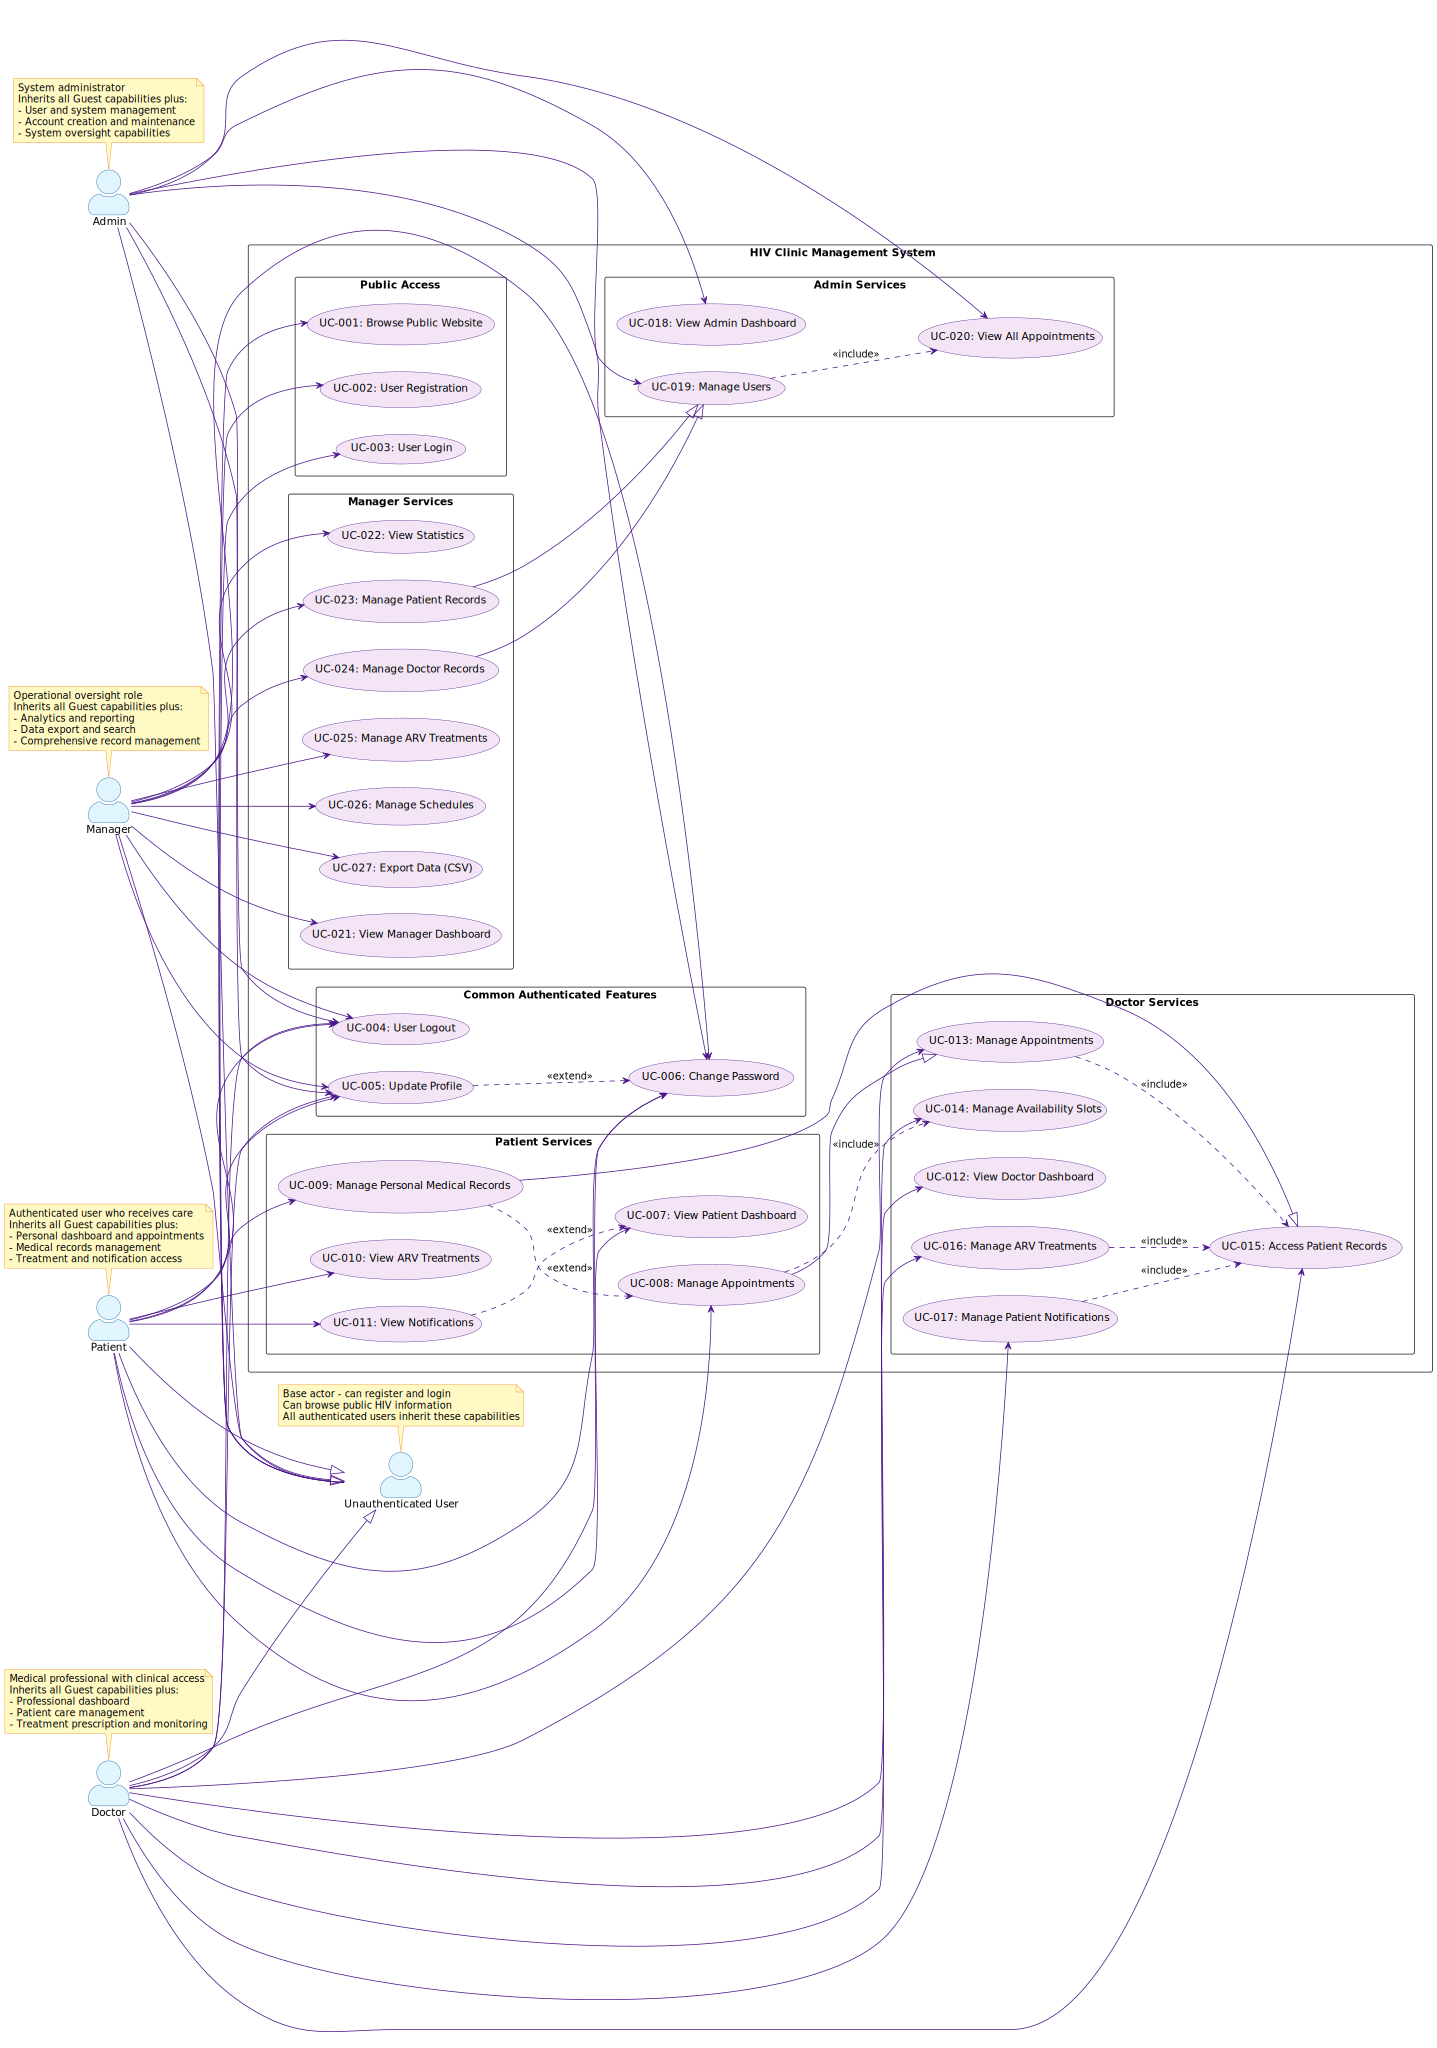
\includegraphics[width=0.9\textwidth]{diagrams/use_case_diagram.png}
\caption{HIV Clinic Management System Use Case Diagram}
\label{fig:use-case-diagram}
\end{figure}

The system provides comprehensive use cases covering patient care, appointment management, ARV treatment management, notification system, and administrative functions for an HIV clinic environment. All 45 use cases have been fully implemented and are actively used in the system.

\paragraph{b. Use Case List}

\begin{longtable}{|c|p{4cm}|p{9cm}|}
\hline
\textbf{UC ID} & \textbf{Use Case Name} & \textbf{Description} \\
\hline
\multicolumn{3}{|c|}{\textbf{Guest/Unauthenticated User Use Cases}} \\
\hline
UC-001 & User Registration & New users create accounts with role-based access \\
\hline
UC-002 & User Login & Users authenticate using username/password \\
\hline
UC-003 & Browse Public Website & Guests access public clinic information \\
\hline
\multicolumn{3}{|c|}{\textbf{Patient Use Cases}} \\
\hline
UC-004 & View Patient Dashboard & Patients access personalized dashboard \\
\hline
UC-005 & Book Appointment & Patients schedule appointments with doctors \\
\hline
UC-006 & View Appointments & Patients view their scheduled appointments \\
\hline
UC-007 & Cancel Appointment & Patients cancel existing appointments \\
\hline
UC-008 & View Medical Records & Patients access their medical history \\
\hline
UC-009 & Update Medical Records & Patients update personal medical information \\
\hline
UC-010 & View ARV Treatments & Patients view prescribed ARV treatments \\
\hline
UC-011 & Update Profile & Patients manage personal profile information \\
\hline
UC-012 & Change Password & Patients update account passwords \\
\hline
UC-013 & Receive Notifications & Patients receive system notifications \\
\hline
UC-014 & View Privacy Settings & Patients manage privacy preferences \\
\hline
\multicolumn{3}{|c|}{\textbf{Doctor Use Cases}} \\
\hline
UC-015 & View Doctor Dashboard & Doctors access professional dashboard \\
\hline
UC-016 & Manage Appointments & Doctors handle appointment scheduling \\
\hline
UC-017 & Update Appointment Status & Doctors modify appointment statuses \\
\hline
UC-018 & Manage Availability & Doctors set available time slots \\
\hline
UC-019 & Access Patient Records & Doctors view patient medical records \\
\hline
UC-020 & Manage ARV Treatments & Doctors prescribe and monitor treatments \\
\hline
UC-021 & Send Notifications & Doctors send messages to patients \\
\hline
UC-022 & Manage Notification Templates & Doctors create reusable message templates \\
\hline
UC-023 & View Notification History & Doctors review sent notifications \\
\hline
\multicolumn{3}{|c|}{\textbf{Administrator Use Cases}} \\
\hline
UC-024 & View Admin Dashboard & Administrators access system overview \\
\hline
UC-025 & Manage Users & Administrators handle user accounts \\
\hline
UC-026 & Create Doctor Accounts & Administrators create professional accounts \\
\hline
UC-027 & Reset User Passwords & Administrators handle password resets \\
\hline
UC-028 & Manage Specialties & Administrators configure medical specialties \\
\hline
UC-029 & Toggle User Status & Administrators activate/deactivate accounts \\
\hline
UC-030 & View All Appointments & Administrators monitor system appointments \\
\hline
\multicolumn{3}{|c|}{\textbf{Manager Use Cases}} \\
\hline
UC-031 & View Manager Dashboard & Managers access operational overview \\
\hline
UC-032 & View Statistics & Managers review system analytics \\
\hline
UC-033 & Manage Patient Records & Managers oversee patient data \\
\hline
UC-034 & Manage Doctor Records & Managers handle doctor information \\
\hline
UC-035 & Manage ARV Treatments & Managers oversee treatment programs \\
\hline
UC-036 & Manage Schedules & Managers coordinate clinic scheduling \\
\hline
UC-037 & Search Patients & Managers find specific patient records \\
\hline
UC-038 & Search Doctors & Managers locate doctor information \\
\hline
UC-039 & Export Data & Managers generate data reports \\
\hline
UC-040 & View Patient Details & Managers access detailed patient views \\
\hline
UC-041 & View Doctor Details & Managers access detailed doctor views \\
\hline
\multicolumn{3}{|c|}{\textbf{System-Wide Use Cases}} \\
\hline
UC-042 & Session Management & System handles user sessions \\
\hline
UC-043 & Login Activity Tracking & System monitors user access \\
\hline
UC-044 & Medication Routine Management & System manages medication schedules \\
\hline
UC-045 & Health Monitoring & System tracks patient health metrics \\
\hline
\end{longtable}

\section{Overall Functionalities}

\subsection{Screens Flow}

The system follows a role-based navigation structure with secure authentication and authorization controls:

\begin{itemize}
    \item \textbf{Public Access}: Guest users can browse public information and register accounts
    \item \textbf{Authentication Gateway}: All users authenticate through secure login
    \item \textbf{Role-Based Dashboards}: Users are redirected to appropriate dashboards based on roles
    \item \textbf{Feature Access Control}: Each role has specific feature access permissions
    \item \textbf{Session Management}: Automatic session timeout and activity tracking
\end{itemize}

\subsection{Screen Descriptions}

\begin{longtable}{|p{4cm}|p{10cm}|}
\hline
\textbf{Screen} & \textbf{Description} \\
\hline
\textbf{Public Homepage} & Landing page with clinic information, services overview, and login/register options \\
\hline
\textbf{Login Screen} & Secure authentication with username/password fields and password reset option \\
\hline
\textbf{Registration Screen} & New user account creation with form validation and terms acceptance \\
\hline
\textbf{Patient Dashboard} & Personalized view with appointments, notifications, and quick actions \\
\hline
\textbf{Doctor Dashboard} & Professional interface with patient management and scheduling tools \\
\hline
\textbf{Admin Dashboard} & System management interface with user administration capabilities \\
\hline
\textbf{Manager Dashboard} & Operational overview with statistics and management functions \\
\hline
\textbf{Appointment Booking} & Interactive calendar with doctor selection and time slot booking \\
\hline
\textbf{Medical Records} & Comprehensive patient health information with privacy controls \\
\hline
\textbf{ARV Treatment Management} & Specialized interface for HIV treatment tracking and monitoring \\
\hline
\textbf{Notification Center} & Message management with filtering and template capabilities \\
\hline
\textbf{Profile Management} & Personal information editing with privacy settings \\
\hline
\textbf{Reporting Interface} & Data visualization and export functionality for managers \\
\hline
\end{longtable}

\subsection{Screen Authorization}

\begin{longtable}{|p{3.5cm}|c|c|c|c|}
\hline
\textbf{Screen/Feature} & \textbf{Patient} & \textbf{Doctor} & \textbf{Admin} & \textbf{Manager} \\
\hline
\textbf{Public Homepage} & X & X & X & X \\
\hline
\textbf{Login/Register} & X & X & X & X \\
\hline
\textbf{Patient Dashboard} & X & & & \\
\hline
\textbf{Doctor Dashboard} & & X & & \\
\hline
\textbf{Admin Dashboard} & & & X & \\
\hline
\textbf{Manager Dashboard} & & & & X \\
\hline
\textbf{Book Appointment} & X & & & \\
\hline
\textbf{View Medical Records} & X & X & & \\
\hline
\textbf{Update Patient Record} & & X & & \\
\hline
\textbf{ARV Treatment Management} & & X & & \\
\hline
\textbf{Medication Routine} & X & X & & \\
\hline
\textbf{Doctor Schedule} & & X & & X \\
\hline
\textbf{Send Notifications} & & X & X & X \\
\hline
\textbf{User Management} & & & X & \\
\hline
\textbf{System Settings} & & & X & \\
\hline
\textbf{Clinical Reports} & & & X & X \\
\hline
\textbf{Notification Management} & & X & X & X \\
\hline
\end{longtable}

\subsection{Non-UI Functions}

\begin{longtable}{|c|p{4cm}|p{8cm}|}
\hline
\textbf{\#} & \textbf{Feature} & \textbf{Description} \\
\hline
1 & Appointment Reminder Service & Automated service sending appointment reminders 24 hours, 1 hour, and 30 minutes before appointments \\
\hline
2 & Medication Reminder Service & Daily service sending medication reminders based on patient routines \\
\hline
3 & Password Reset Service & Automated service handling password reset requests with secure token generation \\
\hline
4 & Database Backup Service & Scheduled service creating regular database backups for data protection \\
\hline
5 & Account Lockout Service & Service monitoring failed login attempts and locking accounts after 6 consecutive failures \\
\hline
6 & Report Generation Service & Service generating clinical and system usage reports for management \\
\hline
7 & Data Validation Service & Service validating and sanitizing user input data for security \\
\hline
8 & Session Management Service & Service handling user session lifecycle and timeout management \\
\hline
\end{longtable}

\section{System High Level Design}

\subsection{Database Design}

\paragraph{a. Database Schema}

The system uses Microsoft SQL Server with the following core tables and relationships:

\begin{longtable}{|c|p{4cm}|p{8cm}|}
\hline
\textbf{No} & \textbf{Table} & \textbf{Description} \\
\hline
01 & Users & Core user table storing all system users with role-based access \\
\hline
02 & Roles & User role definitions for authorization control \\
\hline
03 & PatientProfiles & Extended profile information specific to patients \\
\hline
04 & DoctorProfiles & Extended profile information specific to doctors \\
\hline
05 & Specialties & Medical specialties for categorizing doctors \\
\hline
06 & Appointments & Core appointment booking and management records \\
\hline
07 & DoctorAvailabilitySlots & Doctor schedule and availability management \\
\hline
08 & PatientRecords & Comprehensive patient medical records \\
\hline
09 & ARVTreatments & HIV-specific antiretroviral treatment records \\
\hline
10 & MedicationRoutines & Daily medication schedules with reminder settings \\
\hline
11 & Notifications & System notification management and history \\
\hline
12 & NotificationTemplates & Reusable notification templates for consistency \\
\hline
13 & AppointmentStatusHistory & Audit trail for appointment status changes \\
\hline
14 & AppointmentReminders & Scheduled reminder tracking \\
\hline
15 & SystemHealth & System monitoring and health check data \\
\hline
\end{longtable}

\paragraph{b. Database Diagram}

\begin{figure}[H]
\centering
\includegraphics[width=0.9\textwidth]{diagrams/Picture/Database.png}
\caption{HIV Clinic Database Design}
\label{fig:database-design}
\end{figure}

\subsection{Code Packages}

\begin{longtable}{|c|p{4cm}|p{8cm}|}
\hline
\textbf{No} & \textbf{Package} & \textbf{Description} \\
\hline
01 & controller & REST API controllers handling HTTP requests and responses \\
\hline
02 & service & Business logic layer implementing use cases and workflows \\
\hline
03 & repository & Data access layer for database operations using JPA \\
\hline
04 & model & Entity classes representing database tables with JPA annotations \\
\hline
05 & dto & Data Transfer Objects for API request/response serialization \\
\hline
06 & config & Configuration classes for security, database, and system settings \\
\hline
07 & utils & Utility classes for common operations and helper functions \\
\hline
08 & exception & Custom exception classes for error handling \\
\hline
09 & security & Security-related classes including JWT utilities and filters \\
\hline
10 & validation & Input validation and data sanitization components \\
\hline
\end{longtable}

\subsection{Data Flow Architecture}

\begin{figure}[H]
\centering
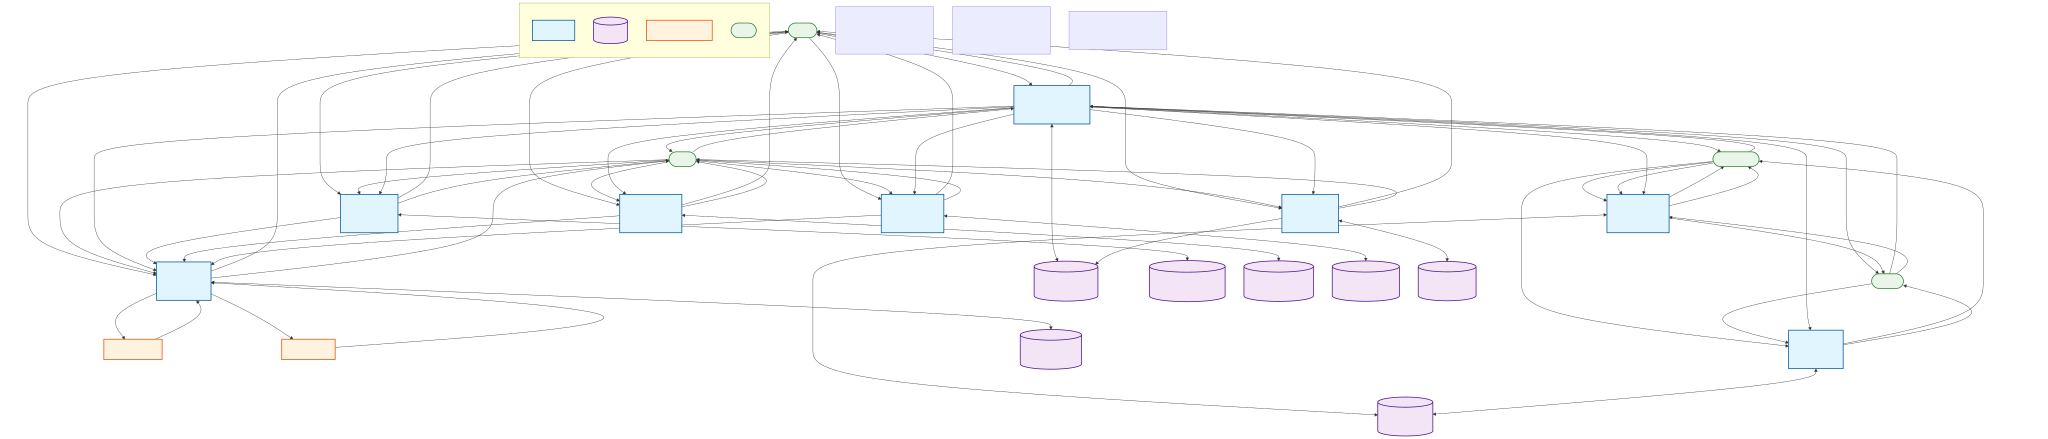
\includegraphics[width=0.9\textwidth]{diagrams/data_flow_diagram.png}
\caption{System Data Flow Diagram}
\label{fig:data-flow-diagram}
\end{figure}

\section{Requirement Specifications}

\subsection{Functional Requirements}

\begin{longtable}{|p{1.2cm}|p{2.5cm}|p{3.5cm}|p{6.8cm}|}
\hline
\textbf{UC ID} & \textbf{Use Case Name} & \textbf{Actor} & \textbf{Functional Requirement} \\
\hline
\multicolumn{4}{|c|}{\textbf{AUTHENTICATION \& USER MANAGEMENT}} \\
\hline
UC-001 & User Registration & Guest & System shall allow new users to create accounts with email validation, password confirmation, and automatic role assignment \\
\hline
UC-002 & User Login & All Users & System shall authenticate users using username/password with JWT token-based security and role-based redirection \\
\hline
\multicolumn{4}{|c|}{\textbf{PUBLIC \& GUEST ACCESS}} \\
\hline
UC-003 & Browse Public Website & Guest & System shall display services information, clinic details, and doctor profiles without requiring authentication \\
\hline
UC-004 & Public Doctor Search & Guest & System shall allow searching and filtering doctors by specialty, name, and availability \\
\hline
\multicolumn{4}{|c|}{\textbf{PATIENT DASHBOARD \& MANAGEMENT}} \\
\hline
UC-004 & View Patient Dashboard & Patient & System shall show appointments, notifications, quick actions, and health summary \\
\hline
UC-005 & Book Appointment & Patient & System shall provide doctor selection, time slot booking, and appointment confirmation \\
\hline
UC-006 & View Appointments & Patient & System shall display scheduled appointments with filtering options \\
\hline
UC-007 & Cancel Appointment & Patient & System shall allow appointment cancellation with confirmation and notification \\
\hline
UC-008 & View Medical Records & Patient, Doctor & System shall display patient medical history with privacy controls \\
\hline
UC-009 & Update Medical Records & Patient & System shall allow patients to update personal medical information \\
\hline
UC-010 & View ARV Treatments & Patient & System shall show prescribed ARV treatments with dosage and schedule information \\
\hline
UC-011 & Update Profile & Patient & System shall allow profile information management including personal details and preferences \\
\hline
UC-012 & Change Password & Patient & System shall provide secure password change with validation \\
\hline
UC-013 & Receive Notifications & Patient & System shall deliver appointment reminders, medication alerts, and general notifications \\
\hline
UC-014 & View Privacy Settings & Patient & System shall allow privacy preference management and record visibility control \\
\hline
\multicolumn{4}{|c|}{\textbf{DOCTOR MANAGEMENT \& PATIENT CARE}} \\
\hline
UC-015 & View Doctor Dashboard & Doctor & System shall display appointments, patients, notifications, and professional summary \\
\hline
UC-016 & Manage Appointments & Doctor & System shall allow appointment viewing, status updates, and patient interaction \\
\hline
UC-017 & Update Appointment Status & Doctor & System shall provide appointment status modification with automatic notifications \\
\hline
UC-018 & Manage Availability & Doctor & System shall allow availability schedule setting and integration with appointment booking \\
\hline
UC-019 & Access Patient Records & Doctor & System shall provide comprehensive patient record access with professional privileges \\
\hline
UC-020 & Manage ARV Treatments & Doctor & System shall allow ARV prescription, monitoring, and treatment plan management \\
\hline
UC-021 & Send Notifications & Doctor & System shall provide notification sending to patients with custom messages \\
\hline
UC-022 & Manage Notification Templates & Doctor & System shall allow creation and management of reusable notification templates \\
\hline
UC-023 & View Notification History & Doctor & System shall provide notification history and delivery status tracking \\
\hline
\multicolumn{4}{|c|}{\textbf{ADMINISTRATIVE FUNCTIONS}} \\
\hline
UC-024 & View Admin Dashboard & Admin & System shall display all system users, appointments, and administrative overview \\
\hline
UC-025 & Manage Users & Admin & System shall provide user detail viewing, editing, and account management \\
\hline
UC-026 & Create Doctor Accounts & Admin & System shall allow doctor account creation with professional information setup \\
\hline
UC-027 & Reset User Passwords & Admin & System shall require password confirmation and provide secure reset functionality \\
\hline
UC-028 & Manage Specialties & Admin & System shall allow medical specialty creation, editing, and assignment management \\
\hline
UC-029 & Toggle User Status & Admin & System shall provide user account activation and deactivation capabilities \\
\hline
UC-030 & View All Appointments & Admin & System shall display system-wide appointment overview with filtering and search \\
\hline
\multicolumn{4}{|c|}{\textbf{MANAGEMENT \& REPORTING}} \\
\hline
UC-031 & View Manager Dashboard & Manager & System shall provide operational dashboards with statistics and management overview \\
\hline
UC-032 & View Statistics & Manager & System shall calculate real-time statistics for appointments, patients, treatments, and system usage \\
\hline
UC-033 & Manage Patient Records & Manager & System shall maintain data integrity and provide comprehensive patient record oversight \\
\hline
UC-034 & Manage Doctor Records & Manager & System shall provide doctor information management and professional record maintenance \\
\hline
UC-035 & Manage ARV Treatments & Manager & System shall monitor treatment effectiveness and provide program oversight capabilities \\
\hline
UC-036 & Manage Schedules & Manager & System shall coordinate clinic-wide scheduling and resource allocation \\
\hline
UC-037 & Search Patients & Manager & System shall support name and ID-based patient search with filtering capabilities \\
\hline
UC-038 & Search Doctors & Manager & System shall integrate with appointment system for doctor search and selection \\
\hline
UC-039 & Export Data & Manager & System shall provide CSV export functionality for reports and data analysis \\
\hline
UC-040 & View Patient Details & Manager & System shall provide comprehensive patient information access for management oversight \\
\hline
UC-041 & View Doctor Details & Manager & System shall provide detailed doctor information and performance metrics \\
\hline
\multicolumn{4}{|c|}{\textbf{SYSTEM-WIDE FUNCTIONS}} \\
\hline
UC-042 & Session Management & System & System shall manage user sessions with timeout controls and security monitoring \\
\hline
UC-043 & Login Activity Tracking & System & System shall track and log user authentication events for security auditing \\
\hline
UC-044 & Medication Routine Management & System & System shall create medication schedules and provide automated reminder services \\
\hline
UC-045 & Health Monitoring & System & System shall monitor patient health metrics and provide alerts for critical conditions \\
\hline
\end{longtable}

\subsection{Non-Functional Requirements}

\begin{longtable}{|p{2.5cm}|p{4cm}|p{7.5cm}|}
\hline
\textbf{Category} & \textbf{Requirement} & \textbf{Specification} \\
\hline
\multicolumn{3}{|c|}{\textbf{PERFORMANCE REQUIREMENTS}} \\
\hline
Response Time & Page Load Time & All pages must load within 3 seconds under normal load conditions \\
\hline
Response Time & API Response Time & All API calls must respond within 2 seconds for 95\% of requests \\
\hline
Throughput & Concurrent Users & System must support at least 100 concurrent users without performance degradation \\
\hline
Throughput & Appointment Booking & System must handle at least 50 appointment bookings per minute during peak hours \\
\hline
\multicolumn{3}{|c|}{\textbf{SECURITY REQUIREMENTS}} \\
\hline
Authentication & Login Security & JWT-based authentication with 30-minute session timeout \\
\hline
Authorization & Role-Based Access & Strict role-based access control with principle of least privilege \\
\hline
Data Protection & Data Encryption & All sensitive data encrypted in transit (HTTPS) and at rest (AES-256) \\
\hline
Password Security & Password Policy & Minimum 8 characters with complexity requirements and regular expiration \\
\hline
\multicolumn{3}{|c|}{\textbf{RELIABILITY REQUIREMENTS}} \\
\hline
Availability & System Uptime & 99.5\% availability during business hours (8 AM - 6 PM) \\
\hline
Data Integrity & Backup Requirements & Daily automated backups with point-in-time recovery capability \\
\hline
Fault Tolerance & Error Handling & Graceful error handling with user-friendly error messages \\
\hline
Disaster Recovery & Recovery Time & System recovery within 4 hours of major failure \\
\hline
\multicolumn{3}{|c|}{\textbf{USABILITY REQUIREMENTS}} \\
\hline
User Interface & Responsive Design & Mobile-responsive design supporting tablets and smartphones \\
\hline
Accessibility & WCAG Compliance & Level AA compliance for users with disabilities \\
\hline
User Experience & Navigation & Intuitive navigation with maximum 3 clicks to reach any feature \\
\hline
Help System & User Support & Context-sensitive help and comprehensive user documentation \\
\hline
\multicolumn{3}{|c|}{\textbf{SCALABILITY REQUIREMENTS}} \\
\hline
User Growth & User Capacity & System must scale to support 1000+ users without architectural changes \\
\hline
Data Growth & Database Scalability & Database design must support 5+ years of patient record growth \\
\hline
Geographic & Multi-location & Architecture must support multiple clinic locations \\
\hline
\multicolumn{3}{|c|}{\textbf{COMPATIBILITY REQUIREMENTS}} \\
\hline
Browser Support & Web Browsers & Chrome 90+, Firefox 88+, Safari 14+, Edge 90+ \\
\hline
Operating System & OS Compatibility & Windows 10+, macOS 10.15+, iOS 13+, Android 8+ \\
\hline
\multicolumn{3}{|c|}{\textbf{COMPLIANCE REQUIREMENTS}} \\
\hline
Healthcare & Medical Standards & HIPAA compliance for patient data privacy and security \\
\hline
Data Privacy & Privacy Regulations & GDPR compliance for data protection and user consent \\
\hline
Medical Records & Clinical Standards & HL7 FHIR compatibility for medical record interoperability \\
\hline
\end{longtable}

\section{Design Specifications}

\subsection{Authentication \& User Management}

\subsubsection{UC-001: User Registration}

\paragraph{a. Functionalities}

\textbf{UC ID and Name:} UC-001: User Registration

\textbf{Created By:} Development Team

\textbf{Date Created:} 06/01/2025

\textbf{Primary Actor:} Guest User

\textbf{Secondary Actors:} System

\textbf{Trigger:} User clicks "Register" link on login page or accesses registration URL

\textbf{Description:} New users can create accounts to access the system. Registration includes email validation, password confirmation, and automatic role assignment based on user type selection.

\textbf{Preconditions:}
\begin{itemize}
\item PRE-1: User has valid personal information
\item PRE-2: Email address is not already registered in the system
\item PRE-3: User has internet connectivity
\end{itemize}

\textbf{Postconditions:}
\begin{itemize}
\item POST-1: New user account is created in the database
\item POST-2: Account activation email is sent to the user
\item POST-3: User profile is created and linked to the account
\item POST-4: Registration activity is logged for audit purposes
\end{itemize}

\textbf{Normal Flow:}
\begin{enumerate}
\item User navigates to registration page
\item System displays registration form with required fields
\item User enters username, email, password, and personal details
\item User selects account type (Patient/Doctor)
\item User agrees to terms and conditions
\item User clicks "Register" button
\item System validates all input fields
\item System checks email uniqueness
\item System creates new user account with appropriate role
\item System generates account activation token
\item System sends activation email
\item System displays registration success message
\end{enumerate}

\textbf{Alternative Flows:}
\begin{itemize}
\item 1.1 Admin Registration: Administrator creates accounts for staff members
\item 1.2 Social Registration: User registers using social media accounts
\end{itemize}

\textbf{Exceptions:}
\begin{itemize}
\item 1.0.E1 Email already registered: System displays error and suggests login
\item 1.0.E2 Invalid email format: System highlights field and shows format requirements
\item 1.0.E3 Password too weak: System displays password strength requirements
\item 1.0.E4 Network error: System retries and shows connection error message
\end{itemize}

\textbf{Priority:} Must Have

\textbf{Frequency of Use:} Medium - New user registrations daily

\textbf{Business Rules:} BR-01, BR-02, BR-03

\textbf{Other Information:} Account activation required within 24 hours

\textbf{Assumptions:} Users have valid email addresses and basic computer literacy

\subsubsection{UC-002: User Login}

\paragraph{a. Functionalities}

\textbf{UC ID and Name:} UC-002: User Login

\textbf{Created By:} Development Team

\textbf{Date Created:} 06/01/2025

\textbf{Primary Actor:} All Users

\textbf{Secondary Actors:} System

\textbf{Trigger:} User accesses protected system resources or login page

\textbf{Description:} Users authenticate to the system using username/password credentials. Upon successful authentication, users are redirected to their role-specific dashboard with appropriate permissions.

\textbf{Preconditions:}
\begin{itemize}
\item PRE-1: User account exists and is active
\item PRE-2: User has valid login credentials
\item PRE-3: Account is not locked due to failed attempts
\end{itemize}

\textbf{Postconditions:}
\begin{itemize}
\item POST-1: User is authenticated and logged into the system
\item POST-2: JWT token is generated and stored for session management
\item POST-3: User session is established with role-based permissions
\item POST-4: Login activity is recorded in audit log
\end{itemize}

\textbf{Normal Flow:}
\begin{enumerate}
\item User accesses the login screen
\item System displays username and password fields
\item User enters credentials
\item User clicks "Login" button
\item System validates credentials against database
\item System verifies account status (active/inactive)
\item System generates JWT token
\item System creates user session with role permissions
\item System records successful login event
\item System redirects to appropriate dashboard based on role
\end{enumerate}

\textbf{Alternative Flows:}
\begin{itemize}
\item 2.1 Password Reset: User clicks "Forgot Password" and follows reset process
\item 2.2 Remember Me: User selects "Remember Me" for extended session
\end{itemize}

\textbf{Exceptions:}
\begin{itemize}
\item 2.0.E1 Invalid credentials: System displays error message and allows retry
\item 2.0.E2 Account locked: System displays lockout message and contact information
\item 2.0.E3 Account inactive: System displays activation required message
\item 2.0.E4 Session timeout: System redirects to login with timeout message
\end{itemize}

\textbf{Priority:} Must Have

\textbf{Frequency of Use:} High - Multiple daily logins per user

\textbf{Business Rules:} BR-04, BR-05, BR-06

\textbf{Other Information:} Session timeout after 30 minutes of inactivity

\textbf{Assumptions:} Users remember their credentials and understand login process

\subsubsection{UC-003: Browse Public Website}

\paragraph{a. Functionalities}

\textbf{UC ID and Name:} UC-003: Browse Public Website

\textbf{Created By:} Development Team

\textbf{Date Created:} 06/01/2025

\textbf{Primary Actor:} Guest User

\textbf{Secondary Actors:} System

\textbf{Trigger:} User visits the clinic website without authentication

\textbf{Description:} Guests can browse public information about the clinic, services offered, doctor profiles, and general health information without requiring account registration or login.

\textbf{Preconditions:}
\begin{itemize}
\item PRE-1: Website is accessible and operational
\item PRE-2: Public content is available and up-to-date
\end{itemize}

\textbf{Postconditions:}
\begin{itemize}
\item POST-1: Public information is displayed to the user
\item POST-2: User has access to registration and login options
\item POST-3: Page visit is logged for analytics
\end{itemize}

\textbf{Normal Flow:}
\begin{enumerate}
\item User visits clinic website URL
\item System displays public homepage
\item User can browse clinic information, services, and doctor profiles
\item User can access health education resources
\item User can view contact information and location details
\item User can navigate to registration or login pages
\end{enumerate}

\textbf{Alternative Flows:}
\begin{itemize}
\item 3.1 Mobile Access: User accesses site via mobile device with responsive design
\item 3.2 Search Engine Access: User finds site through search engine results
\end{itemize}

\textbf{Exceptions:}
\begin{itemize}
\item 3.0.E1 Website unavailable: System displays maintenance message
\item 3.0.E2 Slow connection: System shows loading indicators and progressive content
\end{itemize}

\textbf{Priority:} Must Have

\textbf{Frequency of Use:} High - Daily public website visits

\textbf{Business Rules:} BR-07, BR-08

\textbf{Other Information:} No personal information collected without consent

\textbf{Assumptions:} Users have internet access and modern web browsers

\subsection{Patient Management}

\subsubsection{UC-004: View Patient Dashboard}

\paragraph{a. Functionalities}

\textbf{UC ID and Name:} UC-004: View Patient Dashboard

\textbf{Created By:} Development Team

\textbf{Date Created:} 06/01/2025

\textbf{Primary Actor:} Patient

\textbf{Secondary Actors:} System

\textbf{Trigger:} Patient logs in or navigates to dashboard

\textbf{Description:} Patients access a personalized dashboard displaying appointments, notifications, health summary, and quick action buttons for common tasks.

\textbf{Preconditions:}
\begin{itemize}
\item PRE-1: Patient is logged into the system
\item PRE-2: Patient profile exists and is complete
\item PRE-3: Dashboard data is available and current
\end{itemize}

\textbf{Postconditions:}
\begin{itemize}
\item POST-1: Dashboard is displayed with current patient information
\item POST-2: Recent notifications are marked as viewed
\item POST-3: Dashboard access is logged for activity tracking
\end{itemize}

\textbf{Normal Flow:}
\begin{enumerate}
\item Patient logs in successfully
\item System redirects to patient dashboard
\item System loads patient-specific data
\item System displays upcoming appointments
\item System shows recent notifications
\item System presents health summary with key metrics
\item System provides quick action buttons for common tasks
\item Patient can navigate to detailed features from dashboard
\end{enumerate}

\textbf{Alternative Flows:}
\begin{itemize}
\item 4.1 First Login: System shows welcome tour and setup instructions
\item 4.2 Emergency Alerts: System prominently displays urgent health alerts
\end{itemize}

\textbf{Exceptions:}
\begin{itemize}
\item 4.0.E1 Data loading error: System shows error message and retry option
\item 4.0.E2 No appointments: System suggests booking first appointment
\end{itemize}

\textbf{Priority:} Must Have

\textbf{Frequency of Use:} High - Daily dashboard access

\textbf{Business Rules:} BR-09, BR-10

\textbf{Other Information:} Dashboard refreshes automatically every 5 minutes

\textbf{Assumptions:} Patients understand dashboard layout and icons

\subsubsection{UC-005: Book Appointment}

\paragraph{a. Functionalities}

\textbf{UC ID and Name:} UC-005: Book Appointment

\textbf{Created By:} Development Team

\textbf{Date Created:} 06/01/2025

\textbf{Primary Actor:} Patient

\textbf{Secondary Actors:} Doctor (availability provider), System

\textbf{Trigger:} Patient clicks "Book Appointment" from dashboard or navigation

\textbf{Description:} Patients can view available doctors, their specialties, and time slots, then book appointments with automatic confirmation and reminder scheduling.

\textbf{Preconditions:}
\begin{itemize}
\item PRE-1: Patient is logged in with complete profile
\item PRE-2: At least one doctor has available time slots
\item PRE-3: Patient has no conflicting appointments
\end{itemize}

\textbf{Postconditions:}
\begin{itemize}
\item POST-1: New appointment is created and stored
\item POST-2: Doctor's availability slot is marked as booked
\item POST-3: Confirmation notifications are sent to patient and doctor
\item POST-4: Appointment reminders are automatically scheduled
\end{itemize}

\textbf{Normal Flow:}
\begin{enumerate}
\item Patient accesses appointment booking interface
\item System displays list of available doctors with specialties
\item Patient selects preferred doctor
\item System shows doctor's available time slots
\item Patient selects preferred date and time
\item System displays appointment summary and details
\item Patient confirms appointment booking
\item System creates appointment record
\item System updates doctor's availability
\item System sends confirmation notifications
\item System schedules automated reminders
\item System displays booking confirmation with details
\end{enumerate}

\textbf{Alternative Flows:}
\begin{itemize}
\item 5.1 Reschedule Existing: Patient modifies existing appointment
\item 5.2 Emergency Booking: Patient books urgent appointment with priority
\end{itemize}

\textbf{Exceptions:}
\begin{itemize}
\item 5.0.E1 No available slots: System suggests alternative dates or doctors
\item 5.0.E2 Slot becomes unavailable: System refreshes and shows updated options
\item 5.0.E3 Booking conflict: System alerts and helps resolve scheduling conflict
\end{itemize}

\textbf{Priority:} Must Have

\textbf{Frequency of Use:} High - Multiple daily bookings

\textbf{Business Rules:} BR-11, BR-12, BR-13

\textbf{Other Information:} Appointments can be booked up to 30 days in advance

\textbf{Assumptions:} Patients understand appointment booking process

\section{Appendix}

\subsection{Assumptions \& Dependencies}

\begin{itemize}
\item All users have basic computer literacy and internet access
\item Healthcare providers maintain current medical certifications
\item Patients provide accurate personal and medical information
\item System integrates with existing hospital information systems
\item Network infrastructure supports required bandwidth and security
\end{itemize}

\subsection{Limitations \& Exclusions}

\begin{itemize}
\item Emergency appointment booking outside business hours requires manual intervention
\item System does not provide direct medical advice or diagnosis
\item Integration with external insurance systems is not included in current scope
\item Mobile application development is planned for future releases
\item Telemedicine functionality is excluded from initial implementation
\end{itemize}

\subsection{Business Rules}

\begin{itemize}
\item BR-01: All user accounts require email verification before activation
\item BR-02: Passwords must meet complexity requirements and expire every 90 days
\item BR-03: Patient medical records are private and accessible only to authorized personnel
\item BR-04: Appointment cancellations must be made at least 24 hours in advance
\item BR-05: ARV treatments require doctor prescription and regular monitoring
\item BR-06: System maintains audit logs for all data access and modifications
\end{itemize}

\subsection{Technical Specifications}

\begin{itemize}
\item Backend: Spring Boot 3.0+ with Java 17
\item Frontend: React 18+ with modern JavaScript (ES6+)
\item Database: Microsoft SQL Server 2019+
\item Security: JWT authentication with BCrypt password hashing
\item API: RESTful services with JSON data format
\item Deployment: Docker containers with Kubernetes orchestration
\end{itemize}

\end{document}
